\subsection{Cluster Tracking}
\label{subsec:cluster_tracking}

Once clusters have been identified, it is necessary to track them over consecutive frames to ensure temporal consistency. 
A cluster tracker assigns each detected cluster a unique identifier (ID) and maintains a history of its trajectory over time. 
This enables the system to distinguish between persistent static objects and transient detections caused by noise or dynamic obstacles.

\subsubsection*{Hits and Misses}
Each tracked cluster is updated at every frame using two indices: 
\begin{itemize}
    \item \textbf{Hit Count ($h$):} The number of consecutive frames in which the cluster has been successfully matched to a detection.
    \item \textbf{Miss Count ($m$):} The number of consecutive frames in which the cluster has failed to find a corresponding detection.
\end{itemize}

A cluster is considered \textit{active} if $m \leq M_{\text{max}}$, where $M_{\text{max}}$ is the maximum allowed misses before deletion. 
This mechanism ensures that short occlusions or temporary sensor noise do not cause immediate loss of tracks.

\subsubsection*{Geometric Association}
Let $c_t = (x_t, y_t)$ denote the centroid of a cluster at frame $t$.  
For each existing track, association with a new detection is performed by minimizing the spatial distance:

\begin{equation}
    d(c_t, c_{t+1}) = \lVert c_t - c_{t+1} \rVert_2.
\end{equation}

If a fitted motion model is available, the distance is instead evaluated relative to the predicted cluster trajectory. 
In this project, a simple line-fitting approach was applied to the history of each cluster’s centroids:

\begin{equation}
    y = m x + b,
\end{equation}

where $(m,b)$ are obtained via least-squares regression over the last $N$ centroids.  
The orthogonal distance of a new detection $(x_0, y_0)$ to this fitted line is computed as:

\begin{equation}
    d_{\perp}(x_0, y_0) = \frac{|m x_0 - y_0 + b|}{\sqrt{m^2 + 1}}.
\end{equation}

The detection is associated with the track if $d_{\perp} \leq d_{\text{max}}$, where $d_{\text{max}}$ is a configurable threshold.

\subsubsection*{Track Management}
The complete tracking procedure consists of:
\begin{enumerate}
    \item \textbf{Initialization:} If no tracks exist, each cluster spawns a new track with a unique ID.
    \item \textbf{Association:} Existing tracks are matched to current detections using the minimum distance criterion.
    \item \textbf{Update:} Matched tracks increment their hit count ($h \leftarrow h+1$), reset their miss count, and append the centroid to their history.
    \item \textbf{New Track Creation:} Unmatched detections start new tracks with fresh IDs.
    \item \textbf{Deletion:} Tracks exceeding $M_{\text{max}}$ consecutive misses are deleted.
\end{enumerate}

This process ensures that each stationary object is consistently represented by the same track ID across frames, while spurious detections are naturally filtered out.

\begin{figure}[!htbp]
    \centering
    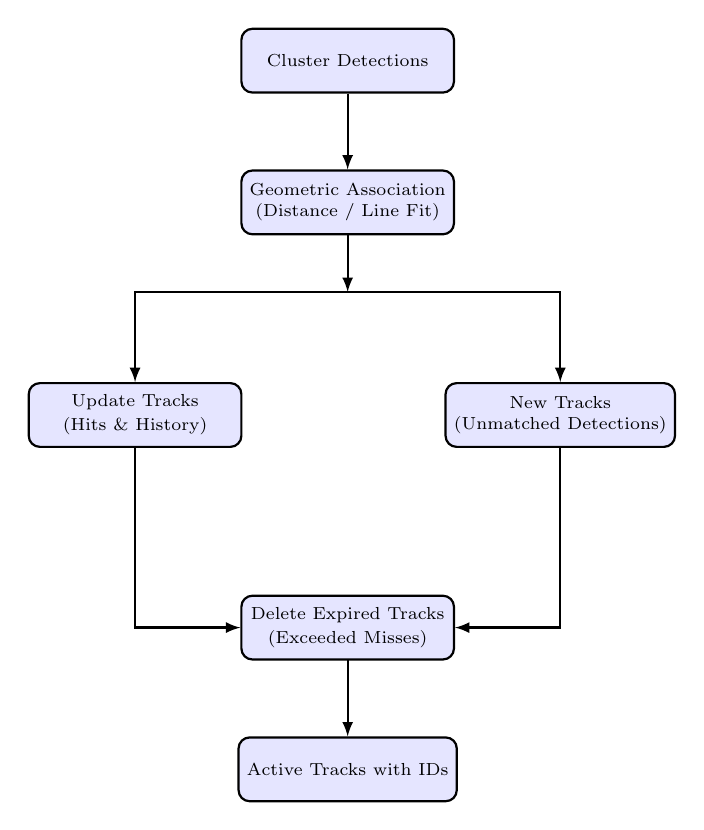
\begin{tikzpicture}[>=latex,thick,scale=0.9, every node/.style={scale=0.9}]
        % Styles
        \tikzstyle{block} = [rectangle, draw, fill=blue!10,
                             rounded corners, minimum height=0.9cm,
                             minimum width=3cm, align=center, font=\scriptsize]
        \tikzstyle{arrow} = [->, thick]

        % ==== Nodes (closer spacing, narrower width) ====
        \node[block] (input)        at (0,0)      {Cluster Detections};
        \node[block] (association)  at (0,-2)     {\shortstack{Geometric Association\\(Distance / Line Fit)}};
        \node[block] (update)       at (-3,-5)    {\shortstack{Update Tracks\\(Hits \& History)}};
        \node[block] (newtrack)     at (3,-5)     {\shortstack{New Tracks\\(Unmatched Detections)}};
        \node[block] (deletion)     at (0,-8)     {\shortstack{Delete Expired Tracks\\(Exceeded Misses)}};
        \node[block] (output)       at (0,-10)    {Active Tracks with IDs};

        % ==== Arrows ====
        \draw[arrow] (input) -- (association);

        % T-branch: down, then split left/right
        \draw[arrow] (association.south) -- ++(0,-0.8) coordinate (branch);
        \draw[arrow] (branch) -| (update.north);
        \draw[arrow] (branch) -| (newtrack.north);

        % Merge toward deletion
        \draw[arrow] (update.south) |- (deletion.west);
        \draw[arrow] (newtrack.south) |- (deletion.east);

        % Final output
        \draw[arrow] (deletion) -- (output);
    \end{tikzpicture}
    \caption{Cluster tracking block diagram. Each detection is associated with existing tracks or used to initialize new tracks. Tracks are deleted after exceeding miss thresholds.}
    \label{fig:cluster_tracking_block}
\end{figure}

To illustrate the method, Figure~\ref{fig:track_cluster_pointcloud} shows a clustered radar point cloud without temporal tracking.  
Figure~\ref{fig:track_cluster_tracked} shows the same scene after applying the tracker: each cluster is assigned an ID, along with Doppler, centroid coordinates, and hit count.  
The tracker maintains these IDs consistently across frames, enabling reliable identification of stationary obstacles.

\begin{figure}[!htbp]
    \centering
    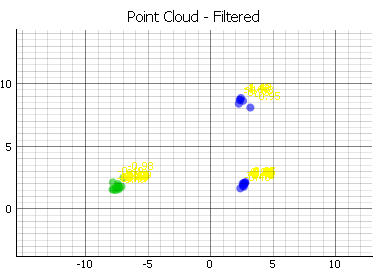
\includegraphics[width=0.48\linewidth]{images/TrackClusterPointCloud.png}
    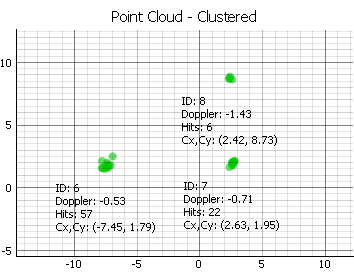
\includegraphics[width=0.48\linewidth]{images/TrackCluster.png}
    \caption{Illustration of the cluster tracking process. Left: clustered point cloud without tracking. Right: tracked clusters with assigned IDs, Doppler values, centroids, and hit counts.}
    \label{fig:track_cluster_pointcloud}
\end{figure}

\vspace{10\baselineskip}